\documentclass[a4paper, 11pt, oneside]{article}

\usepackage[utf8]{inputenc}
\usepackage[T1]{fontenc}
\usepackage[french]{babel}
\usepackage{array}
\usepackage{shortvrb}
\usepackage{listings}
\usepackage[fleqn]{amsmath}
\usepackage{amsfonts}
\usepackage{fullpage}
\usepackage{enumerate}
\usepackage{graphicx}             % import, scale, and rotate graphics
\usepackage{subfigure}            % group figures
\usepackage{alltt}
\usepackage{url}
\usepackage{indentfirst}
\usepackage{eurosym}
\usepackage{listings}
\usepackage{color}
\usepackage[table,xcdraw,dvipsnames]{xcolor}

% Change le nom par défaut des listing
\renewcommand{\lstlistingname}{Extrait de Code}

\definecolor{mygray}{rgb}{0.5,0.5,0.5}
\newcommand{\coms}[1]{\textcolor{MidnightBlue}{#1}}

\lstset{
    language=C, % Utilisation du langage C
    commentstyle={\color{MidnightBlue}}, % Couleur des commentaires
    frame=single, % Entoure le code d'un joli cadre
    rulecolor=\color{black}, % Couleur de la ligne qui forme le cadre
    stringstyle=\color{RawSienna}, % Couleur des chaines de caractères
    numbers=left, % Ajoute une numérotation des lignes à gauche
    numbersep=5pt, % Distance entre les numérots de lignes et le code
    numberstyle=\tiny\color{mygray}, % Couleur des numéros de lignes
    basicstyle=\tt\footnotesize,
    tabsize=3, % Largeur des tabulations par défaut
    keywordstyle=\tt\bf\footnotesize\color{Sepia}, % Style des mots-clés
    extendedchars=true,
    captionpos=b, % sets the caption-position to bottom
    texcl=true, % Commentaires sur une ligne interprétés en Latex
    showstringspaces=false, % Ne montre pas les espace dans les chaines de caractères
    escapeinside={<(}{)>}, % Permet de mettre du latex entre des <( et )>.
    inputencoding=utf8,
    literate=
  {á}{{\'a}}1 {é}{{\'e}}1 {í}{{\'i}}1 {ó}{{\'o}}1 {ú}{{\'u}}1
  {Á}{{\'A}}1 {É}{{\'E}}1 {Í}{{\'I}}1 {Ó}{{\'O}}1 {Ú}{{\'U}}1
  {à}{{\`a}}1 {è}{{\`e}}1 {ì}{{\`i}}1 {ò}{{\`o}}1 {ù}{{\`u}}1
  {À}{{\`A}}1 {È}{{\`E}}1 {Ì}{{\`I}}1 {Ò}{{\`O}}1 {Ù}{{\`U}}1
  {ä}{{\"a}}1 {ë}{{\"e}}1 {ï}{{\"i}}1 {ö}{{\"o}}1 {ü}{{\"u}}1
  {Ä}{{\"A}}1 {Ë}{{\"E}}1 {Ï}{{\"I}}1 {Ö}{{\"O}}1 {Ü}{{\"U}}1
  {â}{{\^a}}1 {ê}{{\^e}}1 {î}{{\^i}}1 {ô}{{\^o}}1 {û}{{\^u}}1
  {Â}{{\^A}}1 {Ê}{{\^E}}1 {Î}{{\^I}}1 {Ô}{{\^O}}1 {Û}{{\^U}}1
  {œ}{{\oe}}1 {Œ}{{\OE}}1 {æ}{{\ae}}1 {Æ}{{\AE}}1 {ß}{{\ss}}1
  {ű}{{\H{u}}}1 {Ű}{{\H{U}}}1 {ő}{{\H{o}}}1 {Ő}{{\H{O}}}1
  {ç}{{\c c}}1 {Ç}{{\c C}}1 {ø}{{\o}}1 {å}{{\r a}}1 {Å}{{\r A}}1
  {€}{{\euro}}1 {£}{{\pounds}}1 {«}{{\guillemotleft}}1
  {»}{{\guillemotright}}1 {ñ}{{\~n}}1 {Ñ}{{\~N}}1 {¿}{{?`}}1
}

%%%%%%%%%%%%%%%%% TITRE %%%%%%%%%%%%%%%%
% Complétez et décommentez les définitions de macros suivantes :
 \newcommand{\intitule}{Rapport puissance 4}
 \newcommand{\GrNbr}{10}
 \newcommand{\PrenomUN}{Jiaxiang}
 \newcommand{\NomUN}{Yao}
 \newcommand{\PrenomDEUX}{Alyssia}
 \newcommand{\NomDEUX}{Kayembe}


%%%%%%%% ZONE PROTÉGÉE : MODIFIEZ UNE DES DIX PROCHAINES %%%%%%%%
%%%%%%%%            LIGNES POUR PERDRE 2 PTS.            %%%%%%%%

\title{INFO0030: \intitule}
\author{Groupe \GrNbr : \PrenomUN~\textsc{\NomUN}, \PrenomDEUX~\textsc{\NomDEUX}}
\date{}

\begin{document}

\maketitle
\newpage
\tableofcontents
\newpage
%%%%%%%%%%%%%%%%%%%% FIN DE LA ZONE PROTÉGÉE %%%%%%%%%%%%%%%%%%%%

%%%%%%%%%%%%%%%% RAPPORT %%%%%%%%%%%%%%%
% Écrivez votre rapport ci-dessous.

\section{Introduction}
Dans le cadre du cours INFO0030, nous avons dû réaliser un projet assez conséquent, marquant, entre autres, la fin de notre 1ère année de Bachelier en Sciences Informatiques.
Ce projet porte sur le développement d'un jeu de Puissance 4 en langage C.
Dans ce rapport, nous allons évoquer l'élaboration de ce programme dans de plus amples détails,
en traitant notamment de l'aspect technique de celui-ci (structures de données, interface graphique, utilisation des ressources, algorithmes, etc.),
 des améliorations que nous aurions faites si nous avions eu plus de temps, mais également de notre expérience en tant qu'équipe,
  la façon dont nous avons géré ce projet et, pour finir, nos apprentissages liés à celui-ci.

\section{Enoncé}

L'énoncé de notre projet nous demandait d'implémenter une version de Puissance 4 dynamique, en appliquant notamment le pattern Modèle-Vue-Contrôleur vu en cours, et en développant un mécanisme permettant au joueur de jouer seul contre l'Ordinateur. De plus, nous devions implémenter le code en C et utiliser \emph{GTK+2} pour l'interface graphique.

\section{Partie technique}

Cette section va traiter des parties plutôt techniques de ce projet, de sa construction à ses mécanismes en passant par sa structure.

\subsection{Architecture générale du code}
L'architecture de notre code se base principalement sur le pattern MVC; \emph{Modèle, Vue et Contrôleur}. Mis à part le pattern MVC, nous avons aussi un fichier code dédié à "l'intelligence artificielle" de notre jeu et un autre dédié à l'interface graphique. Nous en parlerons dans les prochaines sections. Dans cette section, nous allons nous focaliser sur le pattern MVC.

La partie \emph{Modèle} du code recouvre principalement les données et la logique de notre Puissance 4. Parmi les données, nous avons le chemin du fichier contenant les noms des anciens joueurs avec leur score, la taille du plateau du jeu, les informations relatives au joueur courant (telles que son nom, son score, la couleur de ses jetons), les joueurs précédents (et les mêmes informations sur eux), la couleur des jetons de l'I.A. et le mode de jeu. Ces données sont sauvegardées dans une structure. Le \emph{Modèle} comporte également toute la logique du jeu, avec les vérifications et l'intelligence artificielle, la grille représentant l'état du jeu aux yeux du joueur, le fait d'augmenter le score, de mettre en mémoire les données des joueurs précédents contenues dans un fichier, ainsi que la mise à jour de ce même fichier. Nous y retrouvons également pleins de fonctions qui donnent accès aux données.

La \emph{Vue} nous donne une représentation visuelle des données du Modèle. Elle affiche notre plateau de jeu. Elle la change lorsque le joueur décide de placer une jeton, car le Modèle effectue des changements et notifie le Contrôleur (paragraphe suivant) qui lui-même notifie la Vue des changements. La Vue affiche également les labels, notamment avec une message de bienvenue et le score du joueur qui s'incrémente à chaque fois que le joueur place un jeton. Lorsque la partie est terminée, le message de bienvenue va être actualisé pour donner le résultat au joueur.

Le dernier point du pattern MVC concerne le \emph{Contrôleur}, celui-ci gère les entrées du joueur; il informe le Modèle du changement et met à jour la Vue. Le Contrôleur permet au joueur de placer son jeton dans la colonne souhaitée grâce à des boutons, et appelle ensuite les différentes fonctions du \emph{Modèle} reliées à cette action. Il met aussi à jour les labels affichant un message d'information et le score en appelant les fonctions se trouvant dans \emph{Vue}. En outre des labels, il la notifie lorsqu'un pion est ajouté, et celle-ci change une image de la case du plateau de jeu lorsqu'un jeton est placé. En d'autres termes, \emph{Contrôleur} contient toutes les fonctions callbacks, comme celle permettant de recommencer le jeu, et fait office de lien entre le \emph{Modèle} et la \emph{Vue}.

\subsection{Interface graphique}

Pour l'interface graphique de notre Puissance 4, nous utilisons GTK+2. GTK contient une bibliothèque permettant de faire des interfaces graphiques, notamment pour le langage C. 

\begin{figure}[h]
    \center
    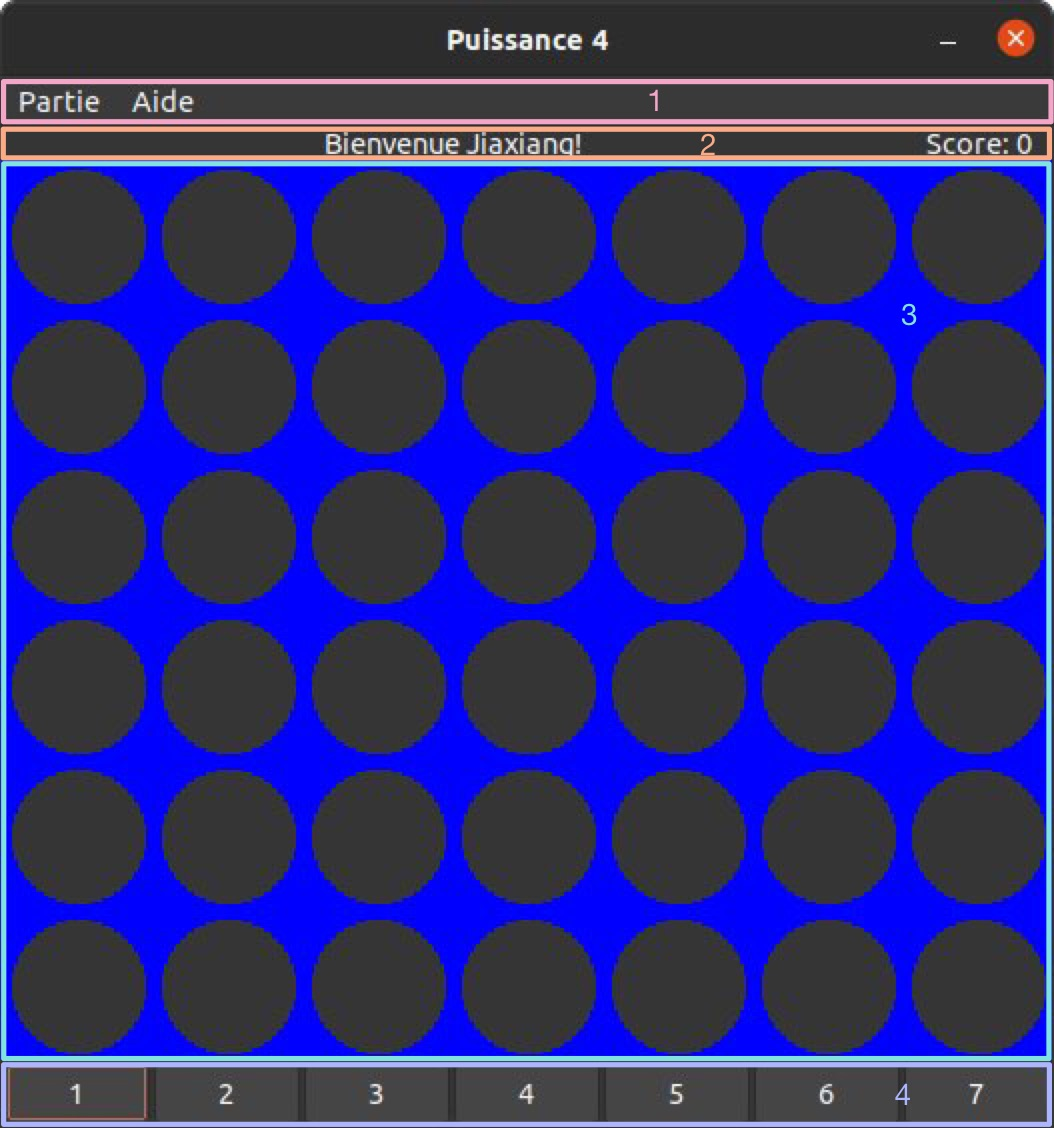
\includegraphics[scale = 0.15]{image1.jpg}
    \caption{L'interface graphique de base du Puissance 4 avec les dimensions par défaut}
\end{figure}


Nous avons utilisé des boxes et des tables pour l'organisation de notre jeu. Cette version du Puissance 4 est composée de 4 zones (cf. FIGURE 1): \\

Notre barre de menu se trouve dans la première zone qui est un GtkVBOX. Elle contient 2 menus principales (cf. FIGURE 2), "Partie" et "Aide", qui peuvent être activés respectivement avec les raccourcis claviers Alt+P et Alt+A. Nous retrouvons dans le menu "Partie", 4 différents items: "Redémarrer une partie", "TOP 10", "Changer le mode du jeu" et "Quitter". Lorsque le joueur clique sur l'item "Redémarrer une partie" ou qu'il utilise le raccourci Ctrl+R, la partie va être réinitialisée et une boîte de dialogue (cf. FIGURE 3) va apparaître pour demander au joueur la couleur du jeton qu'il souhaite. Une boîte de dialogue (cf. FIGURE 3), affichant les 10 meilleurs joueurs avec leur score à côté, apparaît en cliquant sur l'item "TOP 10" ou avec le combo des touches Ctrl+T. Ensuite, l'item "Changer le mode du jeu" permet au joueur de choisir un mode jeu souhaité; soit le mode "classique", ou bien le mode "petit déjeuner". Le joueur peut ainsi choisir le mode de jeu qu'il désire grâce à une boîte de dialogue apparue après avoir activé l'item. Le dernier item du menu "Partie" permet de quitter le jeu et de fermer la fenêtre. Il peut être activé comme les autres en cliquant dessus ou bien en faisant Ctrl+Q. Ensuite, pour le menu "Aide", seul un item est présent; "À propos". Cet item, pouvant être activé en cliquant dessus ou bien avec Ctrl+P, nous donne accès à la boite de dialogue "À propos"(cf. FIGURE 4). Cette boite contient les informations concernant les créateurs de ce programme de Puissance 4.

\newpage

\begin{figure}[h]
    \center
    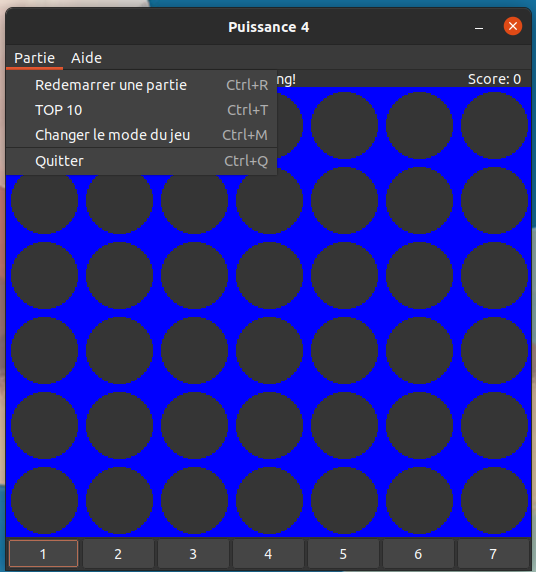
\includegraphics[scale = 0.30]{image2.png}
    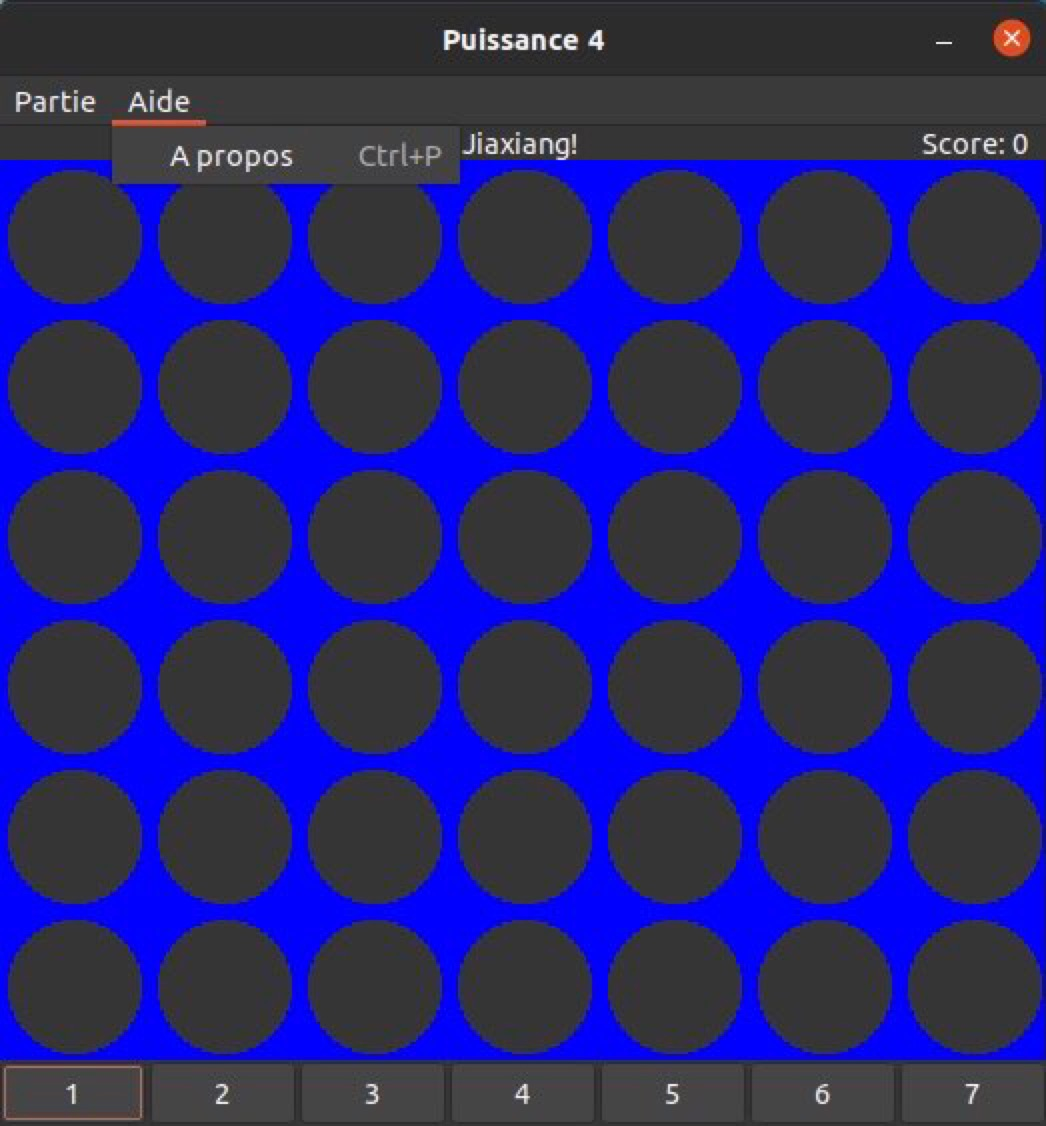
\includegraphics[scale = 0.15]{image3.jpg}
    \caption{Le menu "Partie" à gauche et le menu "Aide" à droite}
\end{figure}

\begin{figure}[h]
    \center
    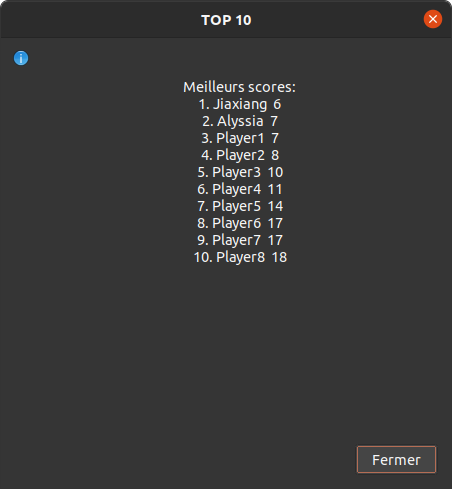
\includegraphics[scale = 0.35]{image4.png}
    
\includegraphics[scale = 0.50]{image5.png}
    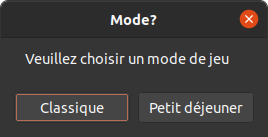
\includegraphics[scale = 0.50]{image10.png}
    \caption{La boite de dialogue "TOP 10" à gauche, la boite de dialogue "Recommencer" au  centre et la boite "Mode" à droite}
\end{figure}

\begin{figure}[!h]
    \center
    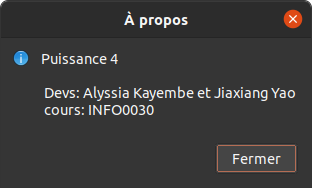
\includegraphics[scale = 0.50]{image6.png}
    \caption{La boite de dialogue "A propos"}
\end{figure}

Dans la zone 2, nous retrouvons une zone dédiée pour les labels qui sont dans un GtkHBox. Celui de gauche affiche un message de bienvenue pour le joueur. Il change quand une partie de jeu est terminée et affiche soit "Vous avez gagné!" si le joueur a gagné, soit "Vous avez perdu..." s'il a perdu, ou encore "Match nul..." si aucun des deux a gagné (cf. FIGURE 5). Nous avons également un autre label à droite, celui-ci affiche le score. Le score s'incrémente à chaque fois que le joueur place un jeton. Si le joueur gagne, le score va être enregistrer dans un fichier texte (si le nom du joueur existe). Lorsque le joueur décide de recommencer une partie, le label du score va être remis à zéro. 

\begin{figure}[!h]
    \center
    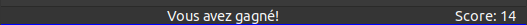
\includegraphics[scale = 0.5]{image7.png}
    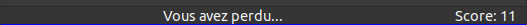
\includegraphics[scale = 0.5]{image8.png}
    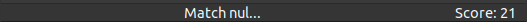
\includegraphics[scale = 0.5]{image9.png}
    \caption{Les différents messages affichés en fonction de du résultat de la partie avec le label du score à droite }
\end{figure}

La zone 3 est la zone du plateau de jeu. Nous avons utilisé un GtkTable pour faire le plateau de jeu. En réalité, le plateau est créé à partir d'une image (bleu.gif) que nous avons mis plusieurs fois, à chaque case de la table, afin d'avoir ce rendu. Lorsque le joueur décide de placer un jeton à un endroit, nous remarquerons qu'un jeton est apparu. En effet, nous avons juste rajouter une image (rouge.gif ou jaune.gif) par dessus à cette case-ci. Comme mentionné au début, le plateau est, en fait, fait à partir d'une table. Cette table a été insérée dans un GtkHBox pour faciliter la ré-initialisation du jeu. Effectivement, le fait de placer la table dans une box rend les choses plus faciles, car lorsque le joueur décide de recommencer une partie, nous avons juste à détruire la table et à le recréer. Nous n'avons pas besoin de détruire le menu, les labels ainsi que les boutons.

La dernière zone est la zone des boutons. Ces boutons permettent au joueur de placer son jeton dans la colonne souhaitée. Ils sont arrangés dans un GtkHbox. Toutefois, le joueur ne sera pas capable de cliquer sur le bouton si la colonne est remplie. De fait, le bouton va être désactivé une fois que la colonne est remplie. De même, tous les boutons vont se désactiver si un des deux joueurs gagne.

Enfin, toutes les GtkHBox citées dans les différents zones sont ensuite arrangées dans la GtkVBox citée dans la partie sur la zone 1.

\subsection{Structures de données}

Nous avons utilisé 3 grandes structures principales pour l'implémentation du programme (MVC), des structures secondaires pour le modèle et des énumérations.

\subsubsection{Model (struct model\_t)}

\hspace{5mm}
\underline{Structure Model:}

\lstinputlisting{struct_model.c}

\hspace{5mm}

Dans la structure Model, il y a d'autres structures qui permettent d'enregistrer des informations plus précises (sur le joueur ou bien sur le mode, par exemple).

\begin{enumerate}
    \item char *highscoresFile: chaîne de caractères contenant le chemin du fichier où se trouve les meilleurs scores;
    \item Colour ** gameGrid: matrice contenant l'état courant de la grille du jeu. Grâce à cette matrice, nous stockons les données du jeu et nous pouvons procéder aux vérifications pour l'I.A. ou pour déterminer si le joueur a gagné;
    \item int *casesLeft: tableau d'entiers contenant l'indice de la ligne dans laquelle sera placé le prochain pion, pour chaque colonne. Ce tableau permet de dire si les pions ont atteint le sommet de la grille dans certaines colonnes, et les cases correspondantes dans le tableau casesLeft valent alors -1;
    \item  unsigned int nbLines: naturel contenant le nombre de lignes de la grille du jeu. Peut être choisi par le joueur;
    \item unsigned int nbColumns. naturel contenant le nombre de colonnes de la grille du jeu. Peut être choisi par le joueur;
    \item User player: structure contenant le données sur le joueur courant.
    Ces données constituent, entre autres, le score du joueur, sa couleur courante, son nom et si celui-ci est présent ou non (la présence du nom détermine la présence du joueur lui-même);
    \item User prevPlayers[NB\_PLAYERS]: tableau de taille statique (NB\_PLAYERS = 10) qui contient les données des 10 joueurs précédents sauvés dans le fichier des meilleurs scores (s'ils existent).
    Les anciens joueurs sont chargés à partir du fichier et imprimés dans la fenêtre pop-up affichant les meilleurs scores;
    \item Colour machineColour: couleur courante de l'Ordinateur qui joue contre le joueur (différente de celle de ce dernier);
    \item Mode mode: variable de type Mode, qui est en réalité une structure contenant les modes du jeu.
    \item []
\end{enumerate}


\hspace{5mm}
\underline{Structure User:}
\lstinputlisting{struct_user.c}
La structure secondaire User permet de stocker des informations sur le joueur.
\begin{enumerate}

    \item name[MAX\_CHAR]: chaîne de caractères représentant le nom d'un joueur. Si elle existe pour le joueur courant et que celui-ci gagne, il sera enregistré dans le fichier des meilleurs scores. 
    \item unsigned int score: le score du joueur. Dans notre programme, ce score sera celui enregistré dans le fichier dans le cas du joueur actuel. Sinon, c'est le score de l'ancien joueur.
    \item Colour colour: couleur du joueur (si ce dernier est un ancien joueur, utilisé pour être placé dans la liste des meilleures scores par exemple, alors la couleur n'est pas forcément nécessaire et peut être initialisée à none [= "aucune"]). 
    \item Boolean present: un booléen permettant d'indiquer si le joueur est présent ou non, c'est-à-dire s'il a rentré un nom ou pas.
    \item []

\end{enumerate}

\hspace{5mm} 
\underline{Structure Mode:}
\lstinputlisting{struct_mode.c}

La structure secondaire mode ne contient qu'un seul champ, Boolean isBreakfast, indiquant si le mode petit déjeuner est activé ou non. Notons que cette structure comportera beaucoup plus de champs si nous décidons de rajouter d'autres modes. \\

\hspace{5mm}
\underline{Enumérations:}
\lstinputlisting{enum.c}

L'énumération Colour comporte 3 constantes: none, red et yellow. Celles-ci sont, en fait, les couleurs des jetons.

L'énumération Result est composée de 3 constantes: lose, win et draw. Ce sont les résultats possibles à la fin d'une partie.

Enfin, l'énumération Boolean contient les constantes false et true, donnant une valeur booléenne.

\subsubsection{View (struct view\_t)}

\hspace{5mm}
\underline{Structure View:}
\lstinputlisting{struct_view.c}

Dans notre structure View, nous avons les champs suivants sauvegardant différentes informations:

\begin{enumerate}
    \item Model *mp: un pointeur sur la structure Model. Ce champ permet à la vue de prendre les données courantes en cas de changements au niveau du modèle.
    \item  GtkWidget *table: la table contenant notre plateau du jeu (images). La taille de la table dépend de celle sauvegardée dans le modèle.
    \item GdkPixbuf *pixBClassic[IMAGES\_NUMBER]: les différentes images utilisées pour le mode classique de notre Puissance 4. Au total, 3 images sont sauvées en mémoire; une case du plateau du jeu, un jeton rouge et un jeton jaune.
    \item GdkPixbuf *pixBToasts[IMAGES\_NUMBER]: les différentes images utilisées pour le mode petit déjeuner. Comme le champ précédent, il comporte au total 3 images; un toast sans confiture, un toast avec de la confiture de fraise et un autre avec de la marmelade d'orange.
    \item GtkWidget *pHBoxGrid: un GtkHBox contenant la table de notre plateau de jeu. Il garde en mémoire la table, citée précédemment, dans une box.
    \item GtkWidget *pLabelScore: le label du score à afficher. Ce label va être actualisé à chaque fois que le joueur ajoute un jeton dans la grille.
    \item GtkWidget *pLabelMessage: le label qui affichera un texte de bienvenue au joueur, à l'état initial, et qui donnera le résultat de la partie. Ce label s'actualise une fois que la partie est terminée.
\end{enumerate}

\subsubsection{Controller (struct controller\_t)}

\hspace{5mm}
\underline{Structure Contrôleur:}
\lstinputlisting{struct_controller.c}

Dans la structure Controller, nous avons les champs suivants:
\begin{enumerate}
    \item Model *mp: un pointeur sur la structure Model. Ce champ permet au contrôleur d'avoir accès au modèle.
    \item  View *vp: un pointeur sur la structure View. Ce champ permet au contrôleur d'avoir accès à la vue.
    \item GdkPixbuf **pGameButtons: les boutons permettant d'ajouter les jetons. Le nombre de boutons dépend du nombre de colonnes et chaque bouton est lié à un événement.
\end{enumerate}

\subsection{Algorithme particulier}
Pour cette version du Puissance 4, le joueur devait pouvoir jouer seul contre l'Ordinateur.
Il fallait donc que notre programme puisse répondre à l'utilisateur de manière cohérente - et ne pas mettre des pions au hasard dans la grille à chaque tour - pour rendre le
jeu un minimum jouable. Il a fallu implémenter une stratégie de jeu en 5 étapes, proposée dans l'énoncé du projet. Il fallait également que le programme puisse détecter un gagnant dans la grille.

Avant même l'élaboration de cette "intelligence artificielle", nous avions déjà pensé à sauver les informations courantes de cette grille à l'aide d'une énumération \texttt{Colour}, définie sur 3 constantes - aucune, rouge et jaune - et à l'aide, surtout, d'une matrice se trouvant dans la structure du modèle. Grâce à cette matrice, notre algorithme pouvait donc se baser sur 2 variables: l'indice de la ligne et de la colonne où se trouve un jeton d'une certaine couleur.

Cependant, le Puissance 4 est un jeu se basant sur la gravité puisque les pions coulissent dans la grille jusqu'à la position la plus basse. De fait, l'ajout de jetons dans la grille devait respecter ce mécanisme. Pour faciliter cette tâche, nous avions donc créé un tableau de la taille du nombre de colonnes (\texttt{CasesLeft[NbColumns]}), initialisé à la position la plus basse et contenant le nombre de cases restantes dans les différentes colonnes avant d'atteindre le sommet de la grille. En d'autres termes, ce tableau contient pour chaque colonne l'indice de la ligne où devra se trouver le prochain jeton si on décide d'ajouter un jeton dans cette colonne. L'indice de la ligne étant, à présent, déterminé par celui de la colonne choisie, notre seule véritable variable est donc l'indice de la colonne.\\


Notre algorithme principal est une fonction prenant plusieurs arguments: la structure du modèle qui contient les structures de données mentionnées ci-dessus, le nombre de pions d'affilée que l'on souhaite vérifier, la couleur que ces pions doivent avoir et un argument particulier permettant de vérifier soit une colonne spécifique, soit toutes les colonnes (si un nombre négatif est donné). Cet algorithme est en réalité une boucle, qui énumère chaque colonne (sauf lorsque l'on souhaite vérifier seulement celle donnée en argument) et inspecte toutes les possibilités de former des séquences de mêmes pions à partir d'un "espace vide" où se trouverait le prochain pion potentiel (l'indice de la ligne pour ce "pion" ou "espace" vide étant donc donné grâce à \texttt{CasesLeft[<colonne>]}). Dès qu'un emplacement est trouvé, la boucle s'arrête et la fonction renvoie l'indice de la colonne où cet emplacement a été détecté.

Pour procéder à cette vérification générale, plusieurs conditions doivent être respectées afin d'éviter les débordements de tableau tout en considérant toutes les directions et tailles que pourraient prendre ces séquences. Les conditions dépendent de la "zone" dans laquelle se trouve le début de la séquence que l'on souhaite vérifier. La gamme donnée en argument détermine la limite de ces zones. Par exemple, si l'on souhaite vérifier une séquence de 3 pions jaunes à la gauche d'une case blanche dans laquelle on souhaiterait placer un autre pion jaune pour gagner, alors l'indice de la colonne où se trouve ce point blanc doit être plus grand ou égal à 3 (cfr. Table \ref{table-1}). Cette condition suffit dans le cas où la direction est horizontale, mais est insuffisante si l'on souhaite vérifier une séquence oblique: il faut également vérifier que le nombre de lignes restantes pour cette colonne soit plus grand ou égal 3 si on souhaite vérifier, par exemple, une séquence à gauche ayant une direction oblique vers le haut (cfr. Table \ref{table-2}).

\begin{table}[h]
\centering
\begin{tabular}{llllllll}
 & 0 & 1 & 2 & 3 & 4 & 5 & 6 \\ \cline{2-8} 
\multicolumn{1}{l|}{0} & \multicolumn{1}{l|}{\cellcolor[HTML]{FE0000}} & \multicolumn{1}{l|}{\cellcolor[HTML]{FE0000}} & \multicolumn{1}{l|}{\cellcolor[HTML]{FE0000}} & \multicolumn{1}{l|}{\cellcolor[HTML]{34FF34}} & \multicolumn{1}{l|}{\cellcolor[HTML]{34FF34}} & \multicolumn{1}{l|}{\cellcolor[HTML]{34FF34}} & \multicolumn{1}{l|}{\cellcolor[HTML]{34FF34}} \\ \cline{2-8} 
\multicolumn{1}{l|}{1} & \multicolumn{1}{l|}{\cellcolor[HTML]{FE0000}} & \multicolumn{1}{l|}{\cellcolor[HTML]{FE0000}} & \multicolumn{1}{l|}{\cellcolor[HTML]{FE0000}} & \multicolumn{1}{l|}{\cellcolor[HTML]{34FF34}} & \multicolumn{1}{l|}{\cellcolor[HTML]{34FF34}} & \multicolumn{1}{l|}{\cellcolor[HTML]{34FF34}} & \multicolumn{1}{l|}{\cellcolor[HTML]{34FF34}} \\ \cline{2-8} 
\multicolumn{1}{l|}{2} & \multicolumn{1}{l|}{\cellcolor[HTML]{FE0000}} & \multicolumn{1}{l|}{\cellcolor[HTML]{FE0000}} & \multicolumn{1}{l|}{\cellcolor[HTML]{FE0000}} & \multicolumn{1}{l|}{\cellcolor[HTML]{34FF34}} & \multicolumn{1}{l|}{\cellcolor[HTML]{34FF34}} & \multicolumn{1}{l|}{\cellcolor[HTML]{34FF34}} & \multicolumn{1}{l|}{\cellcolor[HTML]{34FF34}} \\ \cline{2-8} 
\multicolumn{1}{l|}{3} & \multicolumn{1}{l|}{\cellcolor[HTML]{FE0000}} & \multicolumn{1}{l|}{\cellcolor[HTML]{FE0000}} & \multicolumn{1}{l|}{\cellcolor[HTML]{FE0000}} & \multicolumn{1}{l|}{\cellcolor[HTML]{34FF34}} & \multicolumn{1}{l|}{\cellcolor[HTML]{34FF34}} & \multicolumn{1}{l|}{\cellcolor[HTML]{34FF34}} & \multicolumn{1}{l|}{\cellcolor[HTML]{34FF34}} \\ \cline{2-8} 
\multicolumn{1}{l|}{4} & \multicolumn{1}{l|}{\cellcolor[HTML]{FE0000}} & \multicolumn{1}{l|}{\cellcolor[HTML]{FE0000}} & \multicolumn{1}{l|}{\cellcolor[HTML]{FE0000}} & \multicolumn{1}{l|}{\cellcolor[HTML]{34FF34}} & \multicolumn{1}{l|}{\cellcolor[HTML]{34FF34}} & \multicolumn{1}{l|}{\cellcolor[HTML]{34FF34}} & \multicolumn{1}{l|}{\cellcolor[HTML]{34FF34}} \\ \cline{2-8} 
\multicolumn{1}{l|}{5} & \multicolumn{1}{l|}{\cellcolor[HTML]{FE0000}} & \multicolumn{1}{l|}{\cellcolor[HTML]{FE0000}} & \multicolumn{1}{l|}{\cellcolor[HTML]{FE0000}} & \multicolumn{1}{l|}{\cellcolor[HTML]{34FF34}} & \multicolumn{1}{l|}{\cellcolor[HTML]{34FF34}} & \multicolumn{1}{l|}{\cellcolor[HTML]{34FF34}} & \multicolumn{1}{l|}{\cellcolor[HTML]{34FF34}} \\ \cline{2-8} 
\end{tabular}
\caption{La partie verte représente les cases à partir desquelles on peut vérifier une séquence de 3 éléments horizontales à gauche.}
\label{table-1}
\end{table}

\begin{table}[ht]
\centering
\begin{tabular}{llllllll}
 & 0 & 1 & 2 & 3 & 4 & 5 & 6 \\ \cline{2-8} 
\multicolumn{1}{l|}{0} & \multicolumn{1}{l|}{\cellcolor[HTML]{FE0000}} & \multicolumn{1}{l|}{\cellcolor[HTML]{FE0000}} & \multicolumn{1}{l|}{\cellcolor[HTML]{FE0000}} & \multicolumn{1}{l|}{\cellcolor[HTML]{FE0000}} & \multicolumn{1}{l|}{\cellcolor[HTML]{FE0000}} & \multicolumn{1}{l|}{\cellcolor[HTML]{FE0000}} & \multicolumn{1}{l|}{\cellcolor[HTML]{FE0000}} \\ \cline{2-8} 
\multicolumn{1}{l|}{1} & \multicolumn{1}{l|}{\cellcolor[HTML]{FE0000}} & \multicolumn{1}{l|}{\cellcolor[HTML]{FE0000}} & \multicolumn{1}{l|}{\cellcolor[HTML]{FE0000}} & \multicolumn{1}{l|}{\cellcolor[HTML]{FE0000}} & \multicolumn{1}{l|}{\cellcolor[HTML]{FE0000}} & \multicolumn{1}{l|}{\cellcolor[HTML]{FE0000}} & \multicolumn{1}{l|}{\cellcolor[HTML]{FE0000}} \\ \cline{2-8} 
\multicolumn{1}{l|}{2} & \multicolumn{1}{l|}{\cellcolor[HTML]{FE0000}} & \multicolumn{1}{l|}{\cellcolor[HTML]{FE0000}} & \multicolumn{1}{l|}{\cellcolor[HTML]{FE0000}} & \multicolumn{1}{l|}{\cellcolor[HTML]{FE0000}} & \multicolumn{1}{l|}{\cellcolor[HTML]{FE0000}} & \multicolumn{1}{l|}{\cellcolor[HTML]{FE0000}} & \multicolumn{1}{l|}{\cellcolor[HTML]{FE0000}} \\ \cline{2-8} 
\multicolumn{1}{l|}{3} & \multicolumn{1}{l|}{\cellcolor[HTML]{FE0000}} & \multicolumn{1}{l|}{\cellcolor[HTML]{FE0000}} & \multicolumn{1}{l|}{\cellcolor[HTML]{FE0000}} & \multicolumn{1}{l|}{\cellcolor[HTML]{34FF34}} & \multicolumn{1}{l|}{\cellcolor[HTML]{34FF34}} & \multicolumn{1}{l|}{\cellcolor[HTML]{34FF34}} & \multicolumn{1}{l|}{\cellcolor[HTML]{34FF34}} \\ \cline{2-8} 
\multicolumn{1}{l|}{4} & \multicolumn{1}{l|}{\cellcolor[HTML]{FE0000}} & \multicolumn{1}{l|}{\cellcolor[HTML]{FE0000}} & \multicolumn{1}{l|}{\cellcolor[HTML]{FE0000}} & \multicolumn{1}{l|}{\cellcolor[HTML]{34FF34}} & \multicolumn{1}{l|}{\cellcolor[HTML]{34FF34}} & \multicolumn{1}{l|}{\cellcolor[HTML]{34FF34}} & \multicolumn{1}{l|}{\cellcolor[HTML]{34FF34}} \\ \cline{2-8} 
\multicolumn{1}{l|}{5} & \multicolumn{1}{l|}{\cellcolor[HTML]{FE0000}} & \multicolumn{1}{l|}{\cellcolor[HTML]{FE0000}} & \multicolumn{1}{l|}{\cellcolor[HTML]{FE0000}} & \multicolumn{1}{l|}{\cellcolor[HTML]{34FF34}} & \multicolumn{1}{l|}{\cellcolor[HTML]{34FF34}} & \multicolumn{1}{l|}{\cellcolor[HTML]{34FF34}} & \multicolumn{1}{l|}{\cellcolor[HTML]{34FF34}} \\ \cline{2-8} 
\end{tabular}
\caption{La partie verte représente les cases à partir desquelles on peut vérifier une séquence de 3 éléments obliques en haut à gauche}
\label{table-2}
\end{table}

En considérant toutes les directions que peuvent prendre ces séquences dans cette grille, nous obtenons 8 séquences possibles: verticales (au dessus ou en dessous), horizontales (à droite ou à gauche), et obliques (vers le haut ou vers bas \textbf{et} vers la droite ou vers la gauche). Notons qu'il est inutile de vérifier le cas où des pions se trouveraient à la verticale au dessus du pion d'origine, c'est-à-dire du pion "vide", puisque aucun pion ne peut se retrouver au dessus de lui. Nous obtenons donc différentes conditions propres à chacune de ces 7 situations. Pour les implémenter, nous comparons alors les zones définies grâce à la gamme avec l'indice de la colonne et/ou celui de la ligne du lieu où devra se trouver le prochain jeton, et cela directement dans les fonctions \textbf{verify} nécessitant certaines de ces conditions. Ainsi, nous évitons les dépassements de tableau. Notons également que nous n'allons pas exposer en détail les cas où un pion pourrait se retrouver entre plusieurs pions de même couleur comme nous venons de le faire, mais que ces cas suivent le même principe que ci-dessus en modifiant légèrement la comparaison (on diminue la gamme d'une unité et on vérifie les cas particuliers où un des indices se trouve sur les bords de la grille) et sont aussi considérés par notre algorithme (et représentés par trois des fonctions verify).

Toutes nos fonctions de vérifications (\texttt{verify\_[...]}) sont au nombre de 10 et implémentées dans un fichier à part nommé ai.c. Elles sont toutes appelées dans la fonction \texttt{check\_grid} et vérifient toutes les possibilités de séquences qui pourraient être formées. Pour cela, elles prennent comme argument l'indice de la colonne à vérifier, la grille, le tableau contenant les indices pour les lignes, la couleur à vérifier, la gamme et, quand besoin est, le nombre de colonnes et/ou de lignes. Chaque fonction vérifie une ou plusieurs situations (si elles sont assez similaires)  qui pourraient survenir. Par exemple, \texttt{verify\_left} vérifie pour chaque colonne la situation représentée ci-dessus par la Table 1, tandis que \texttt{verify\_up\_left} s'occupe de celle représentée par la Table 2.

Il serait intéressant de souligner le fait que les 7 premières fonctions \texttt{verify}, cherchant une séquence d'une certaine taille, sont assez générales et peuvent servir pour tout type de gamme. Cependant, les 3 dernières fonctions (\texttt{verify\_within\_...}) ont été créées pour servir aux cas particuliers où un pion pourrait se retrouver entre d'autres pions de même couleur. À cause de cela, ces fonctions sont moins modulaires pour ce qui est du choix de la gamme, celle-ci devant valoir 2 ou 3 (si ce n'est pas le cas, les fonctions renvoient automatiquement -1). Nous avons décider de les garder ainsi car il n'était pas nécessaire de les rendre plus modulaires, et que nous souhaitions travailler sur d'autres aspects du projet.

Pour terminer cette sous-section traitant de notre algorithme particulier, nous souhaitions souligner la particularité de notre fonction \texttt{check\_grid}. En effet, celle-ci peut ainsi couvrir toutes les vérifications nécessaires grâce à une série d'arguments. Elle peut être appelée pour vérifier si un joueur est sur le point de gagner en plaçant son jeton dans une certaine colonne, on donne alors comme argument la couleur du joueur, une gamme qui vaut 3 et l'indice de la colonne dans laquelle celui-ci est sur le point de placer son pion. La fonction peut également servir à l'I.A. pour vérifier si elle-même à la possibilité de faire un puissance 4, de bloquer le joueur s'il peut en faire un également (dans ces deux cas, seule la couleur diffère et la gamme vaut toujours 3), d'empêcher le joueur d'ajouter un troisième pion pour former une séquence de 3 jetons ou, à l'opposé, de se permettre elle-même d'en mettre un de sa couleur lorsque l'occasion de faire de même se présente (dans ces deux autres cas, la couleur diffère aussi mais la gamme vaut 2). Dans tous les cas, pour ce qui est de l'argument demandant une colonne spécifique, un nombre négatif sera donné à la fonction \texttt{check\_grid}, puisque nous voulons vérifier toutes les possibilités pour chacune des colonnes de la grille. C'est d'ailleurs ce que notre fonction \texttt{add\_token\_ai} s'occupe de faire, entre autres. Celle-ci regroupe les 4 situations sous forme d'étapes à suivre, et si aucune de ces étapes n'est fructueuse, elle prend l'indice d'une colonne aléatoire qui n'est pas encore remplie (les étapes sont celles décrites dans l'énoncé du projet pour le déroulement du jeu). En outre, la fonction \texttt{check\_grid} avait été créée exprès pour l'I.A., d'où notre décision d'ajouter un argument supplémentaire, quitte à ne l'utiliser qu'une seule fois dans le programme, plutôt que de créer 4 boucles successives directement dans la fonction \texttt{add\_token\_ai} ou bien 4 fonctions différentes assez répétitives.

\subsection{Analyse de performance}
Pour ce projet, il nous était demandé de réaliser un profiling et une analyse des performances de notre code. 

Pour le profiling, nous avons utilisé l'outil de profilage \emph{gprof}. Nous avons effectué 6 tests (2 pour chaque situation possible) et observé que la fonction la plus appelée est la fonction \texttt{check\_height} avec en moyenne 505.625 appels lors de nos tests. Ensuite, les fonctions les plus appelées sont toutes les autres fonctions \texttt{check\_[...]} se trouvant dans le fichier ai.c, suivies de \texttt{get\_nbColumns}. Cela a du sens, car notre code en général dépend énormément du nombre de colonnes (qui représente le nombre d'itérations que la boucle de notre fonction \texttt{check\_grid} effectue lorsque l'on souhaite vérifier toute la grille).

Ensuite, pour ce qui est de la quantité de ressources utilisées, nous avons calculé la valeur de chaque champs que nous avons ensuite additionné pour chaque structure correspondante. Voici ce que nous obtenons:
\begin{itemize}
    \item Pour calculer le nombre de ressources que la structure model\_t utilise, nous avons calculé tous les champs individuellement, y compris ceux des structures secondaires, et nous obtenons le polynôme suivant:
    $$744 + 4 \times (C) \times (L + 1)$$
    avec C représentant le nombre de colonnes et L représentant le nombre de lignes. Les ressources consommées pour cette structure dépendent donc de ces deux inconnues. Si les tailles sont mises par défaut, avec C = 7 et L = 6, alors la structure consommera 940 bytes. Cette valeur est la quantité minimale de ressources que cette structure peut consommer, les tailles par défaut ne pouvant être plus petites. Remarquons que cette structure consomme une quantité importante de ressources due au fait que nous donnons une taille statique, qui est assez grande (MAX\_CHAR = 50), aux chaînes de caractères \emph{name}.
    
    \item Ensuite, pour le nombre de ressources utilisé par la structure vue\_t, nous avons rajouté une ligne de code, \texttt{printf("\%ld\textbackslash n", sizeof(View))}, pour obtenir le nombre de bytes utilisés. Suite à cela, nous constatons que cette structure consomme bien en tout 88 bytes. En effet, chacun de nos champs représente 8 bytes et si nous faisons le calcule, nous avons $$ 8 + 8 + (8  * 3)+ (8 * 3) + 8 + 8 + 8 = 88$$.
    Le résultat obtenu correspond bien à ce que la fonction \texttt{sizeof()} nous a fourni.
    
    \item Enfin, le contrôleur contient deux adresses, celle d'une variable sur View et une autre sur Model, mais aussi un tableau de taille variable contenant les pointeurs sur GtkWidget pour les boutons. La structure, non initialisée, consomme ainsi 24 bytes. Lorsque la taille est donnée à la création, nous obtenons ce polynôme:
    $$16 + 8 * C$$
    avec C représentant le nombre de colonnes que contient la grille du jeu. Si cette variable C est laissée par défaut, elle vaudra alors 7, ce qui signifie que la structure créée dans une variable de type \texttt{Controller} consommera environ 72 bytes. Cette valeur est la quantité minimale de ressources qui seront consommées par le programme pour le contrôleur, mais cette valeur peut donc augmenter en fonction du choix du joueur.
\end{itemize}

Nous avons calculé le temps consommé dans l'une de nos fonctions, \texttt{click\_button\_game(GtkWidget *pButton, gpointer data)}, qui est censée être la fonction qui consomme le plus de temps. Nous remarquons que le temps d'exécution est quasi inexistant lorsque nous sommes en pleine partie. Par conséquent, nous pouvons tirer comme conclusion que notre complexité temporelle est assez correcte. Même lorsque nous augmentons le nombre de lignes et de colonnes, cela n'influence pas le temps d'exécution de la fonction, ou bien de façon très minime à notre niveau.
\section{Travail d'équipe}

Cette section va traiter de notre expérience en tant que binôme pour ce projet, de notre coopération et de la gestion du projet (avec le SCM).

\subsection{Coopération}
Ce projet était à faire en binôme. Le nôtre s'est beaucoup basé sur la communication et le partage. Nous avons toutes les deux les mêmes méthodes de travail, ce qui nous facilitait la tâche pour ce qui était de la collaboration. En effet, nous étions dans le même état d'esprit et avions les mêmes idées pour tout ce qui concernait l'organisation de notre code (et en particulier sa propreté). Nous avons essayé de nous occuper d'un peu tous les aspects du projet en général, mêmes si nous avions des tâches et des rôles spécifiques pour l'élaboration de ce projet.

Pour la répartition du travail, les tâches principales de Jiaxiang touchaient tout ce qui concernait l'implémentation de l'interface, de la Vue ainsi que de l'ensemble des tests tandis qu'Alyssia s'est chargée du Modèle, d'une majorité du backend et des mécanismes permettant au programme de fonctionner sur le fond. Nous avons toutes les deux collaborées sur l'intelligence artificielle et sur le Contrôleur.

De fait, nous avons réfléchi ensemble à l'intelligence artificielle que nous souhaitions implémenter (ce qui était probablement la partie la plus importante pour ce projet), en écrivant sur papier tous les cas possibles, en discutant de l'implémentation, des problèmes qui pouvaient survenir en fonction de la situation et des façons de rendre le code propre.

De manière générale, nous avons réparti le travail en misant sur les points forts et les points faibles de chacune, tout en nous entraidant mutuellement lorsque l'une de nous éprouvait des difficultés, et ce fut une expérience et une collaboration enrichissantes.

\subsection{Gestion du code}

Pour le SCM, nous avons utilisé le Gitlab de l'Université de Liège (https://gitlab.uliege.be) pour gérer le code de notre projet. Nous avons chacune travaillé sur nos machines respectives et nous avons beaucoup utilisé le Git. Il est vrai que cela était difficile à utiliser au début, mais une fois que les commandes ont été apprises et utilisées quelques fois, le Git s'est avéré extrêmement efficace et rapide. Il nous a fait gagner énormément de temps durant le projet. Il est devenu aisé de s'échanger du code ou de procéder aux tests sur différentes machines. Cela était aussi très rassurant de savoir qu'il y avait une copie de notre projet stockée quelque part si quoi que ce soit devait arriver.

Pour ce qui est de notre utilisation du Git, habituellement nous essayions de commit après avoir fini certaines modifications spécifiques puis nous faisions un push une fois que l'on avait terminé de travailler ou avant de faire une pause. Il est vrai que nous ne faisions pas tout le temps cela, et que parfois nous nous échangions du code directement via le git en effectuant des petites modifications et plusieurs commits peu significatifs pour celles-ci, ou bien il se pouvait que l'une d'entre nous oubliait de push son travail, mais en général cela restait assez rare et nous avons tenté, au mieux, de garder une certaine habitude quant à l'utilisation du SCM.

\section{Améliorations éventuelles}

Si nous avions disposé de plus de temps pour effectuer ce projet, nous aurions probablement tenté, d'abord, d'améliorer notre Intelligence Artificielle, par exemple en parcourant toutes les positions en comptant, pour chaque colonne, et en sauvegardant dans un tableau à l'indice associé, le nombre de possibilités/avantages que représente l'ajout d'un pion potentiel dans la colonne en question. Tout cela en donnant un certain poids aux différentes actions possibles. Par exemple, l'action d'empêcher le joueur de former une séquence de 4 pions aurait un poids 10x plus élevé que celle qui permettrait à la machine d'ajouter un 3e pion.

Nous aurions probablement ajouté un système de sauvegarde également, se basant sur nos projets précédents (sauvegarde en mémoire d'un fichier PNM et création de code-barres images). En effet, nous aurions probablement ajouté une option (optionnelle) lors du lancement du programme, ou bien une option dans le menu, qui aurait alors appelé une fonction chargée de mettre en mémoire les dimensions de la grille en début de fichier, le score, la couleur du joueur, et les différentes données pour notre structure de donnée \texttt{casesLeft[nbColumns]}. Puis, cette fonction aurait lu la grille dans ce même fichier pour la placer en mémoire dans le modèle. Ensuite, nous aurions simplement appelé notre fonction \texttt{initialise\_images} qui se serait chargée du reste pour ce qui est de la partie visuelle de la grille.
Pour ce qui est de la sauvegarde du fichier, nous aurions utilisé le même principe que la fonction \texttt{write\_pnm} du projet 1.

Enfin, nous aurions ajouté plus de modes pour le jeu, ajoutés dans la structure \texttt{Mode} implémentée dans model.c. Par exemple, des modes avec  de nouvelles images à thèmes, une option qui active ou non de la musique, etc. En outre, nous avions pensé à implémenter un mode multijoueur, que nous avons réussi à mettre en place dans le cadre de nos tests. Malheureusement, par manque de temps et par soucis de propreté, nous avons décidé de ne pas ajouter ce mode afin d'avoir plus de temps quant au peaufinement du reste du code et du rapport.

\section{Apprentissages}

Ce projet nous a appris et apporté beaucoup:

\begin{itemize}
    \item Tout d'abord, il nous a appris à travailler en groupe. Nous avions du mal à nous organiser au début, mais au fur et à mesure, nous avons réussi à trouver des moyens efficaces pour collaborer. Nous avons également appris l'organisation et la communication au sein de ce binôme;
    
    \item Nous avons appris à gérer un peu mieux nos deadlines, et à mieux gérer notre stress par rapport à celles-ci, en nous fixant des petits objectifs à atteindre toutes les deux à certaines dates;
    
    \item De plus, nous maîtrisons mieux les pointeurs. En effet, nous manipulons beaucoup de pointeurs pour ce projet, et nous nous y sommes habituées. Cela nous apporte beaucoup dans notre apprentissage du C.

    \item Nous avons appliqués les diverses méthodes vues au cours d'INFO0030, notamment pour ce qui est du SCM (cfr. 4.2 Gestion du code) et du débogage (avec gbd et \texttt{printf("\%\textbackslash d", \_\_LINE\_\_)} ) que nous avons vraiment pus mettre en pratique grâce à ce projet;

    \item Finalement, nous avons appris que nous étions capables de réaliser des projets d'une telle envergure, malgré la difficulté que ce projet représentait pour nous au début. Nous avons appris concrètement ce qu'était la programmation cette année, et nous sommes très fières d'avoir pû mettre en pratique toutes nos connaissances accumulées au cours de celle-ci, afin de pouvoir enfin admirer le fruit de notre travail.
\end{itemize}

\section{Conclusion}

Pour conclure ce rapport, rappelons l'objectif de notre programme qui était d'implémenter un jeu de Puissance 4 dynamique, en langage C et avec la librairie \emph{GTK+2}. Ce rapport décrit en détail les aspects techniques de notre code, mais reprend également notre ressenti face à ce projet. Bien qu'imparfait, nous sommes fières de ce que nous avons produit et des apprentissages que nous avons pu tirer de celui-ci.

\end{document}
